\section{Fragmentation}

\pgfdeclareimage[width=1.0\paperwidth]{header-image}{header_images/helicopter}
%\againframe<5->{framework}


\begin{frame}<2>[label=controlMaps]
    \frametitle{So Humans have no impact on fire?}
    \framesubtitle{Suppression}
    \controlsSide{limitation_map}
\end{frame}

\pgfdeclareimage[width=1.0\paperwidth]{header-image}{header_images/Mirador_de_Garbi}
\begin{frame}
    \frametitle{So Humans have no impact of fire?}
    \framesubtitle{Fragmentation}
    \begin{textblock*}{11cm}(0cm,1.5cm)
    \visible<1->{
    	\begin{tikzpicture}
    	\node[anchor=north,inner sep=0] (image) at (0,0) {
    		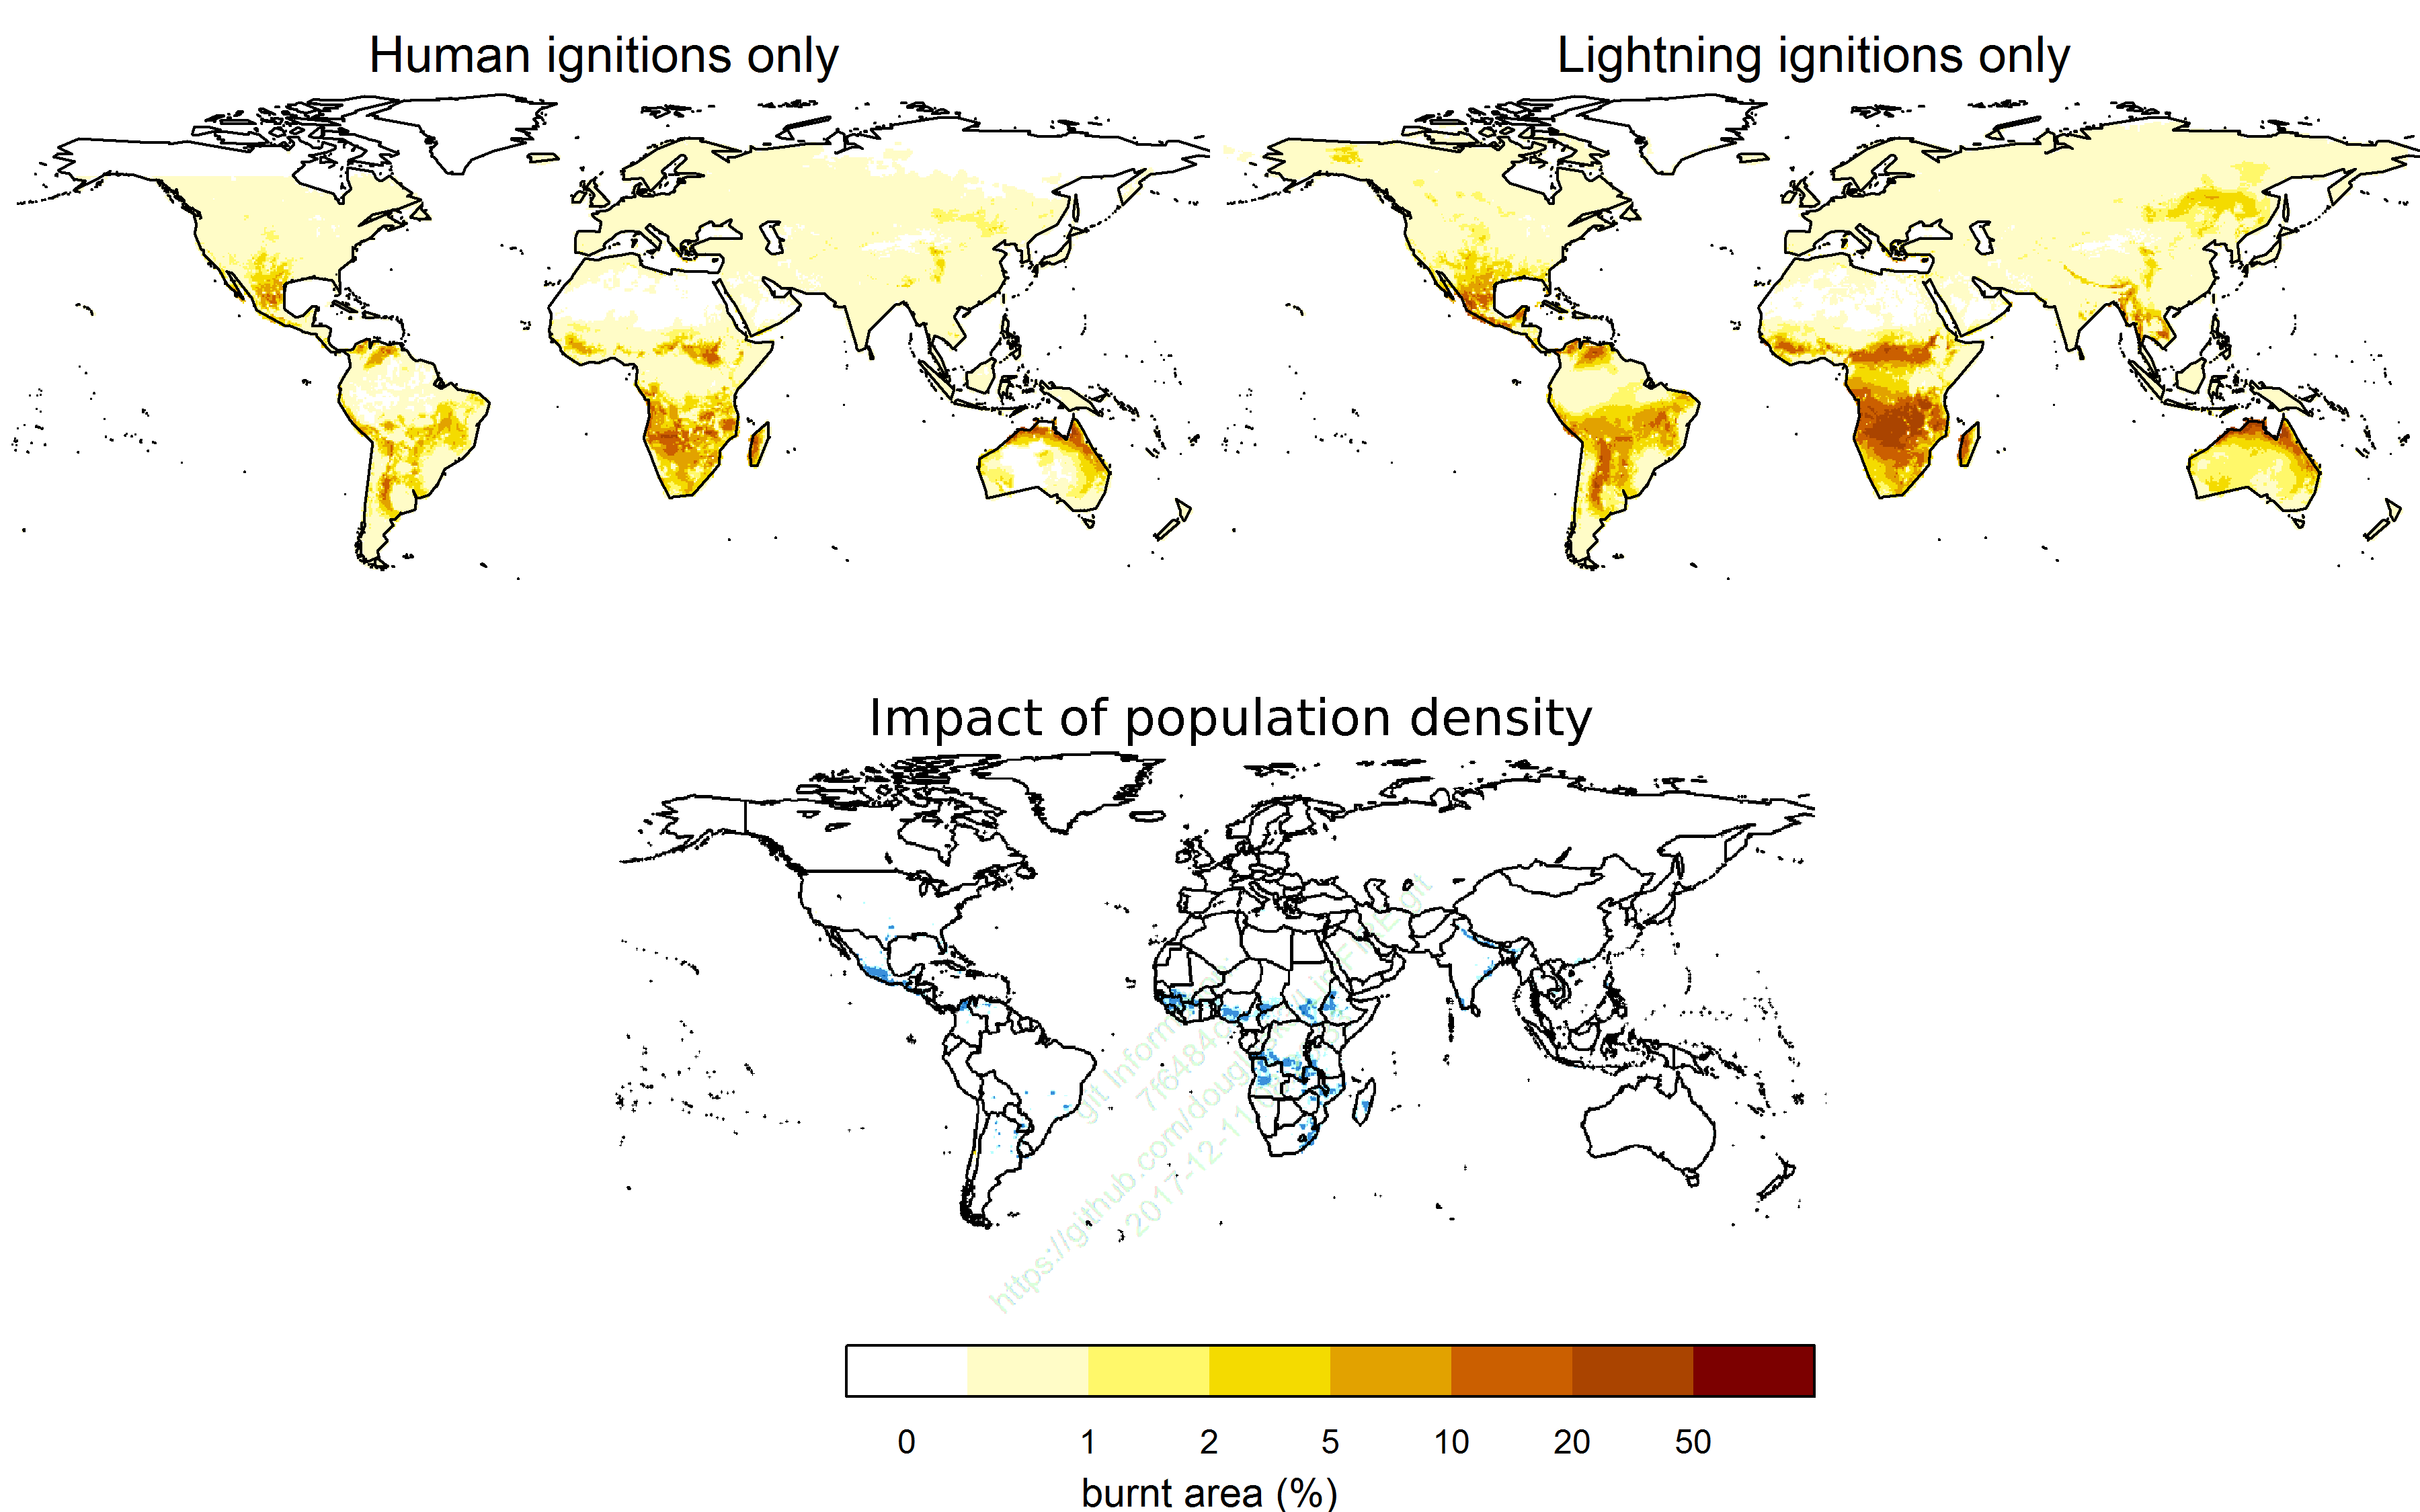
\includegraphics[trim={5.1cm 2cm 5.1cm 6.2cm},clip,width=6.2cm]{images/igntitions/IgntionInfoSourceAdding}
	    };
        \node[anchor=south,align=center] at (0, -0.2) {Human Ignitions};
        \end{tikzpicture}
    }
	%trim = {l b r t}
    \visible<2->{
    	\begin{tikzpicture}
    	\node[anchor=north,inner sep=0] (image) at (0,0) {
    		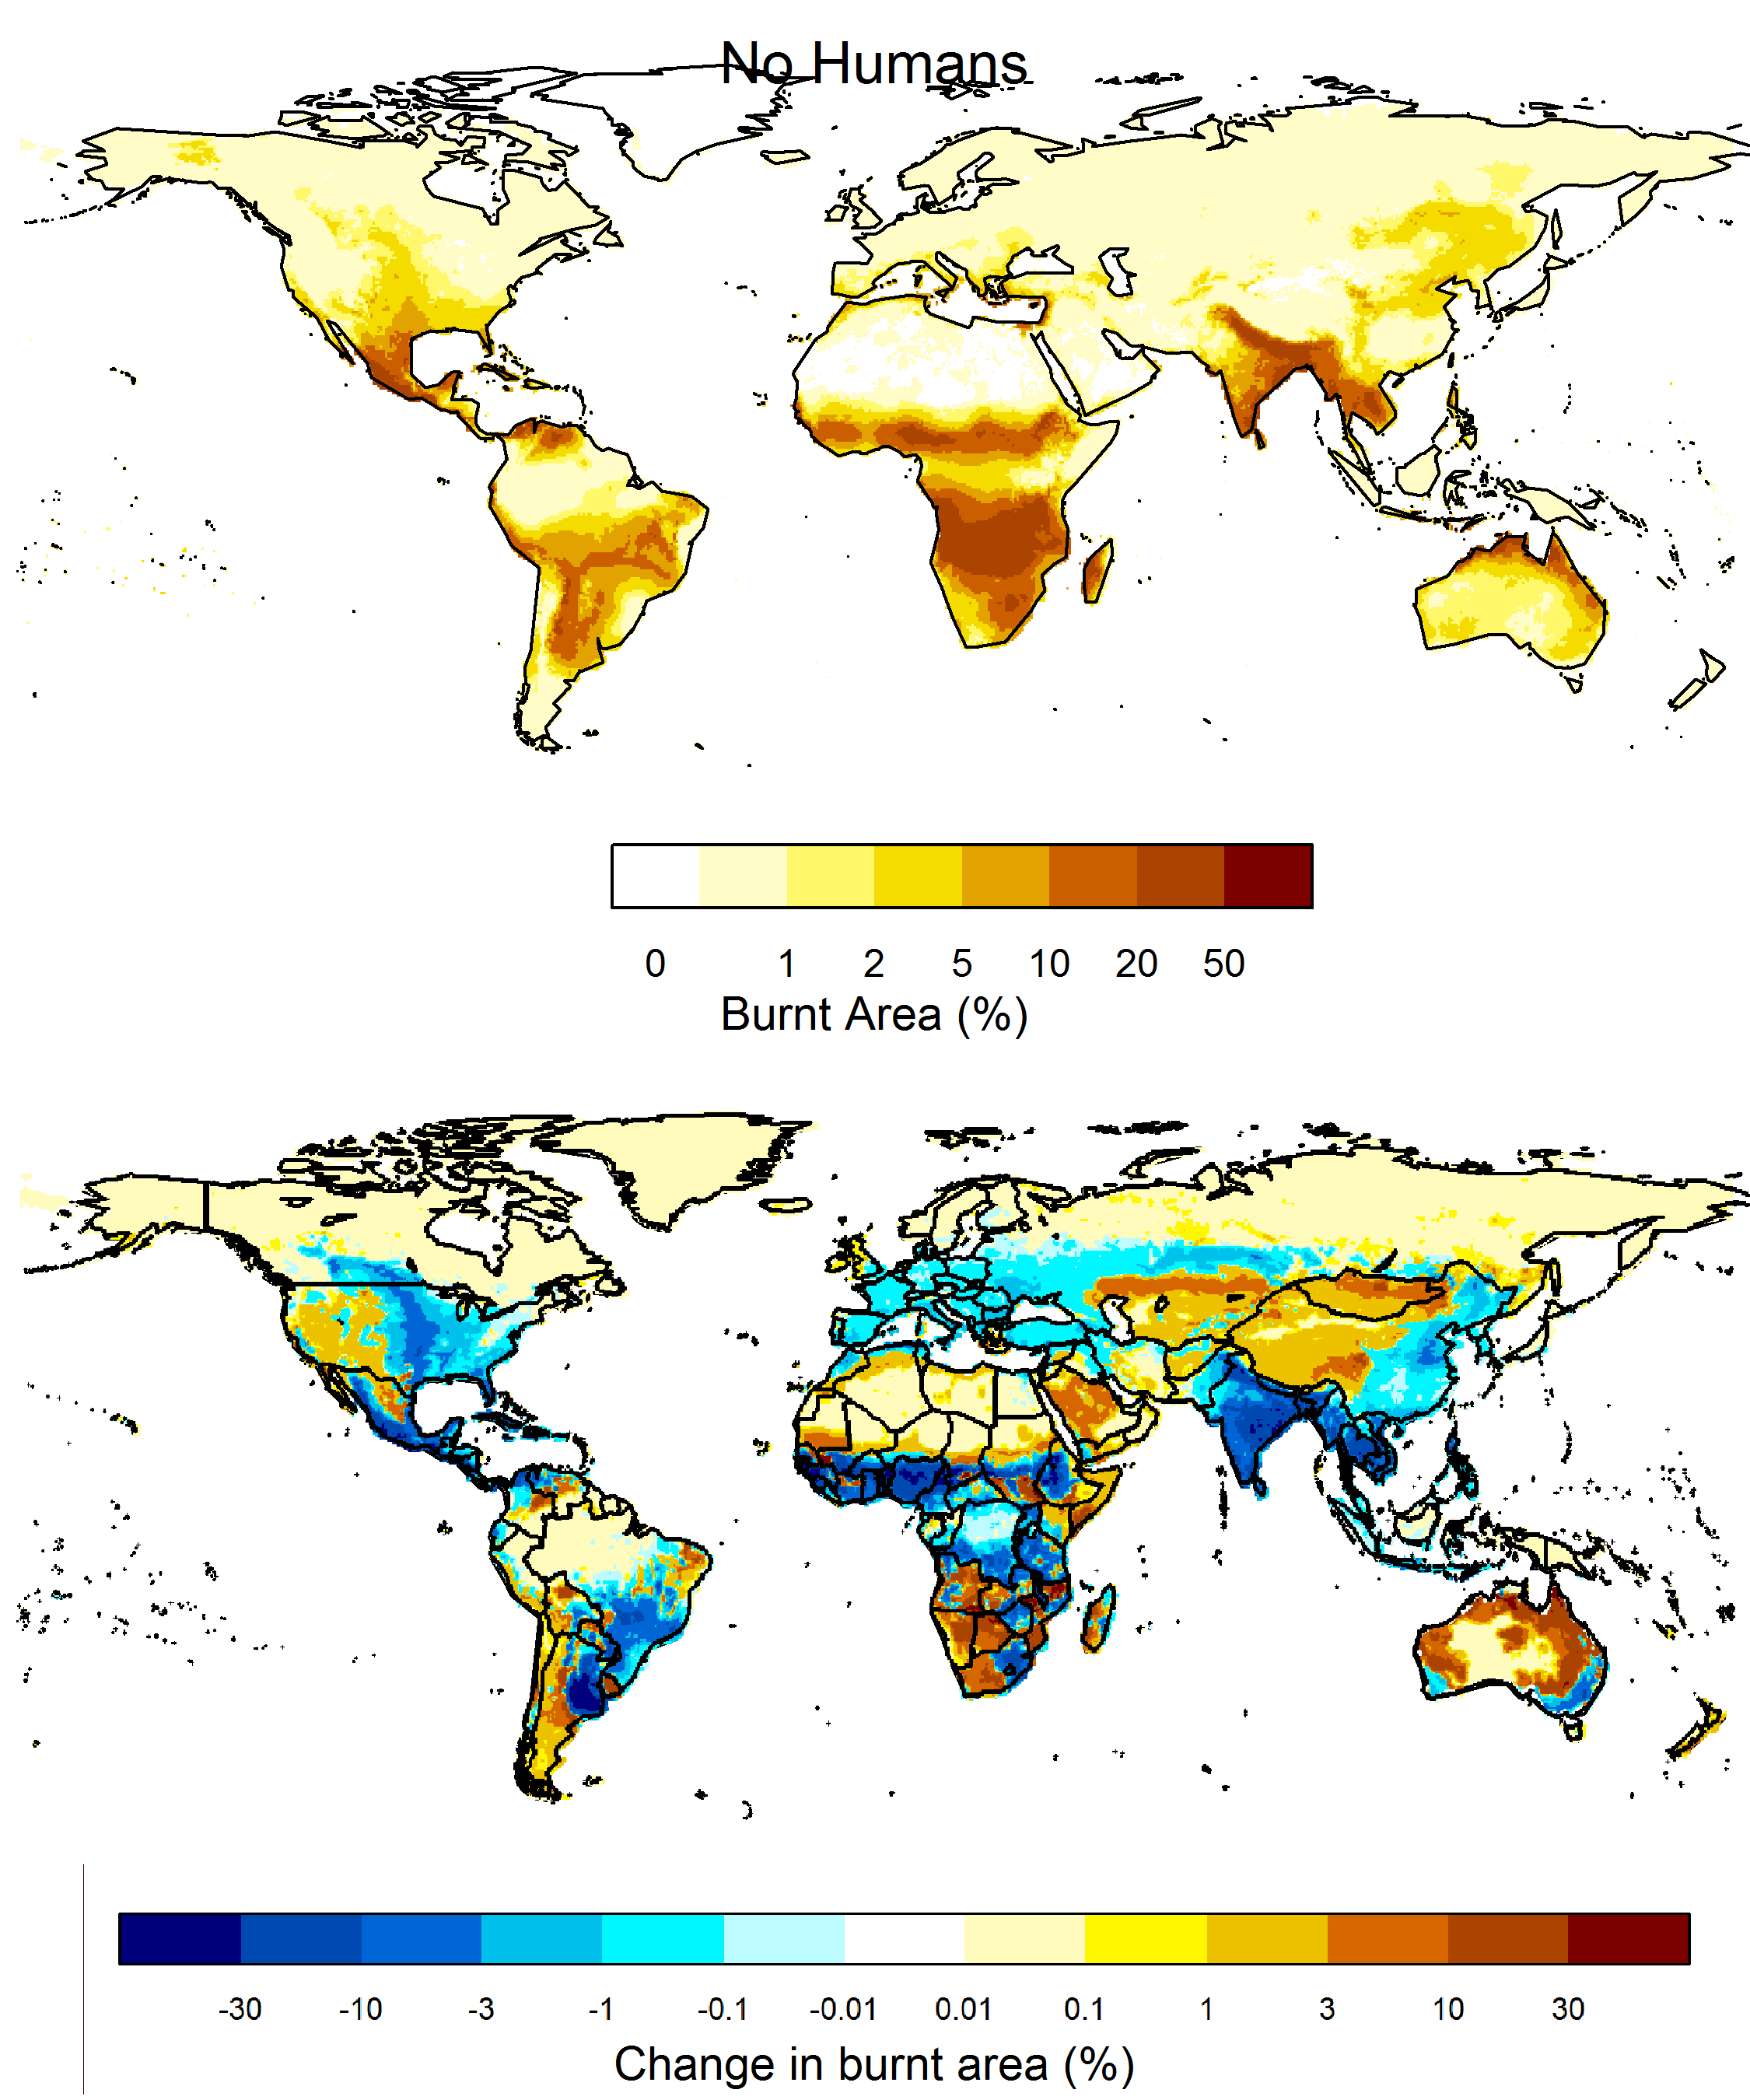
\includegraphics[trim={0 0 0 8cm},clip,width=6.2cm]{images/igntitions/IgntionInfoNoHumans}
    	};
    	\node[anchor=south,align=center] at (0, -0.2) {Overall Human Impact};
    	\end{tikzpicture}
        
    }
    \end{textblock*}
    \begin{textblock*}{11cm}(6.4cm,1.3cm)
    \visible<3->{
        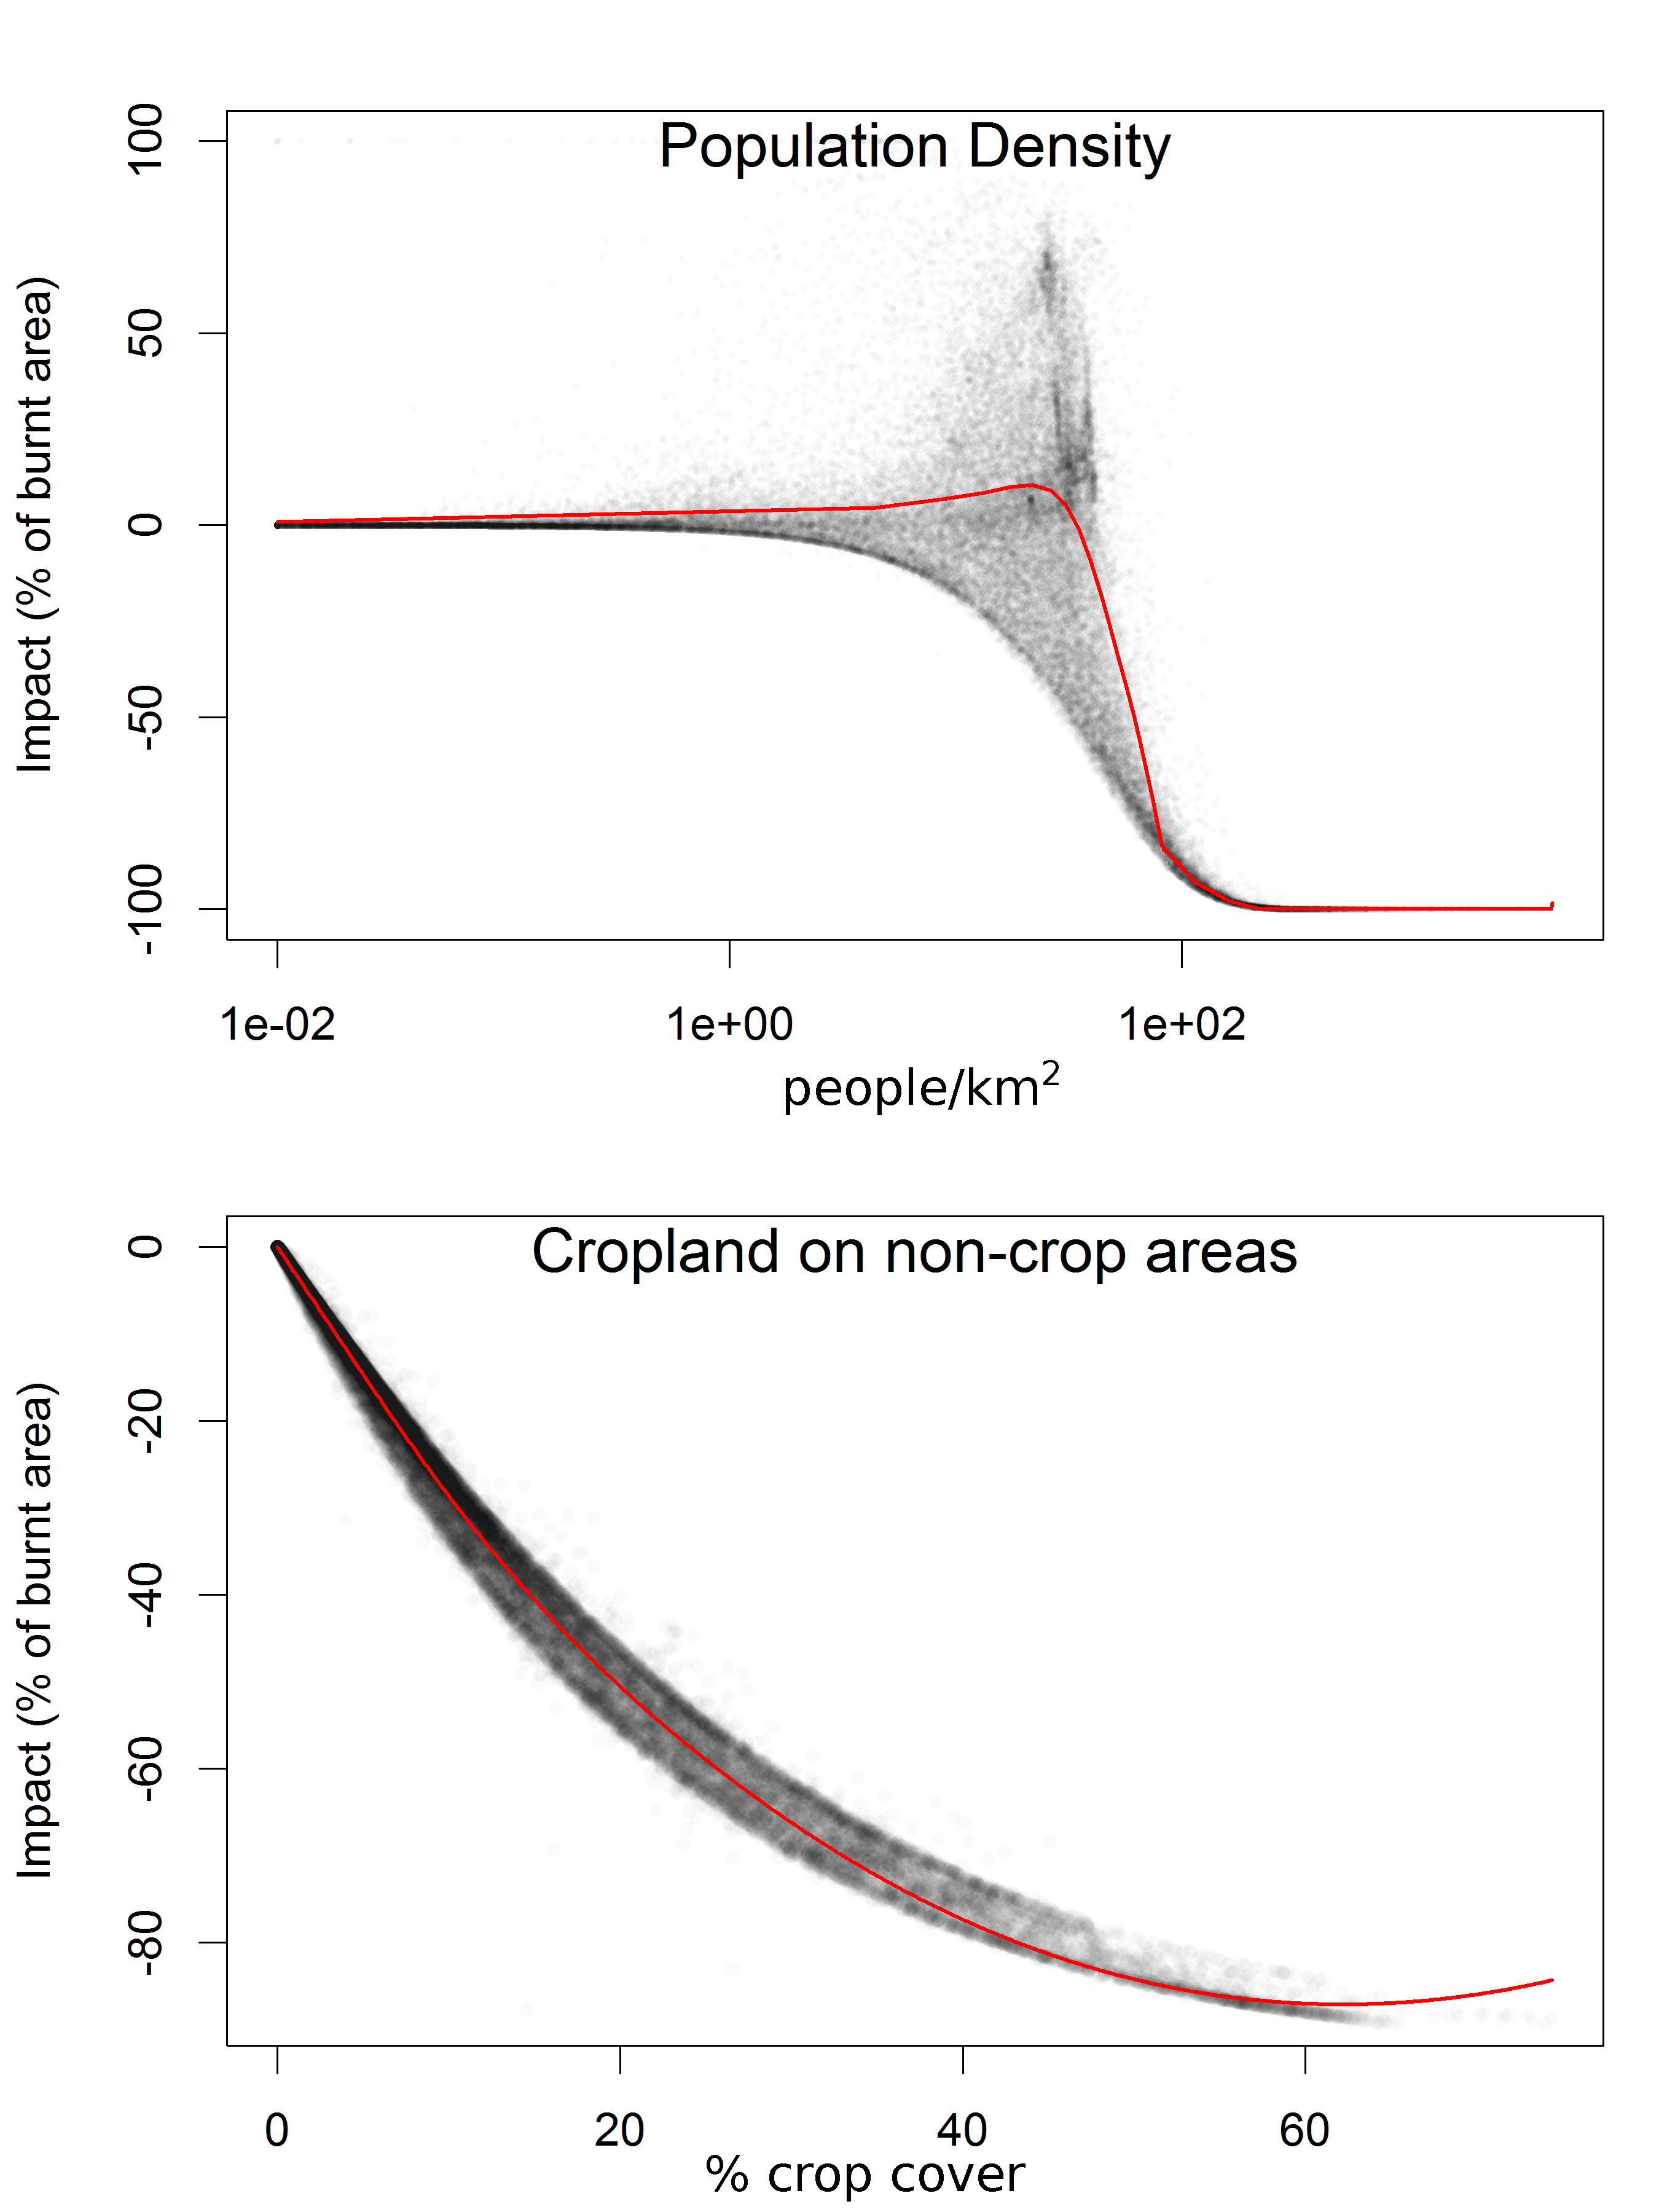
\includegraphics[width=5.5cm]{images/human_noHuman_impact}
    }
    \end{textblock*}

    %\visible<3->{
    %    \begin{tikzpicture}
    %        \node[anchor=south west,inner sep=0] (image) at (0,0) {
    %            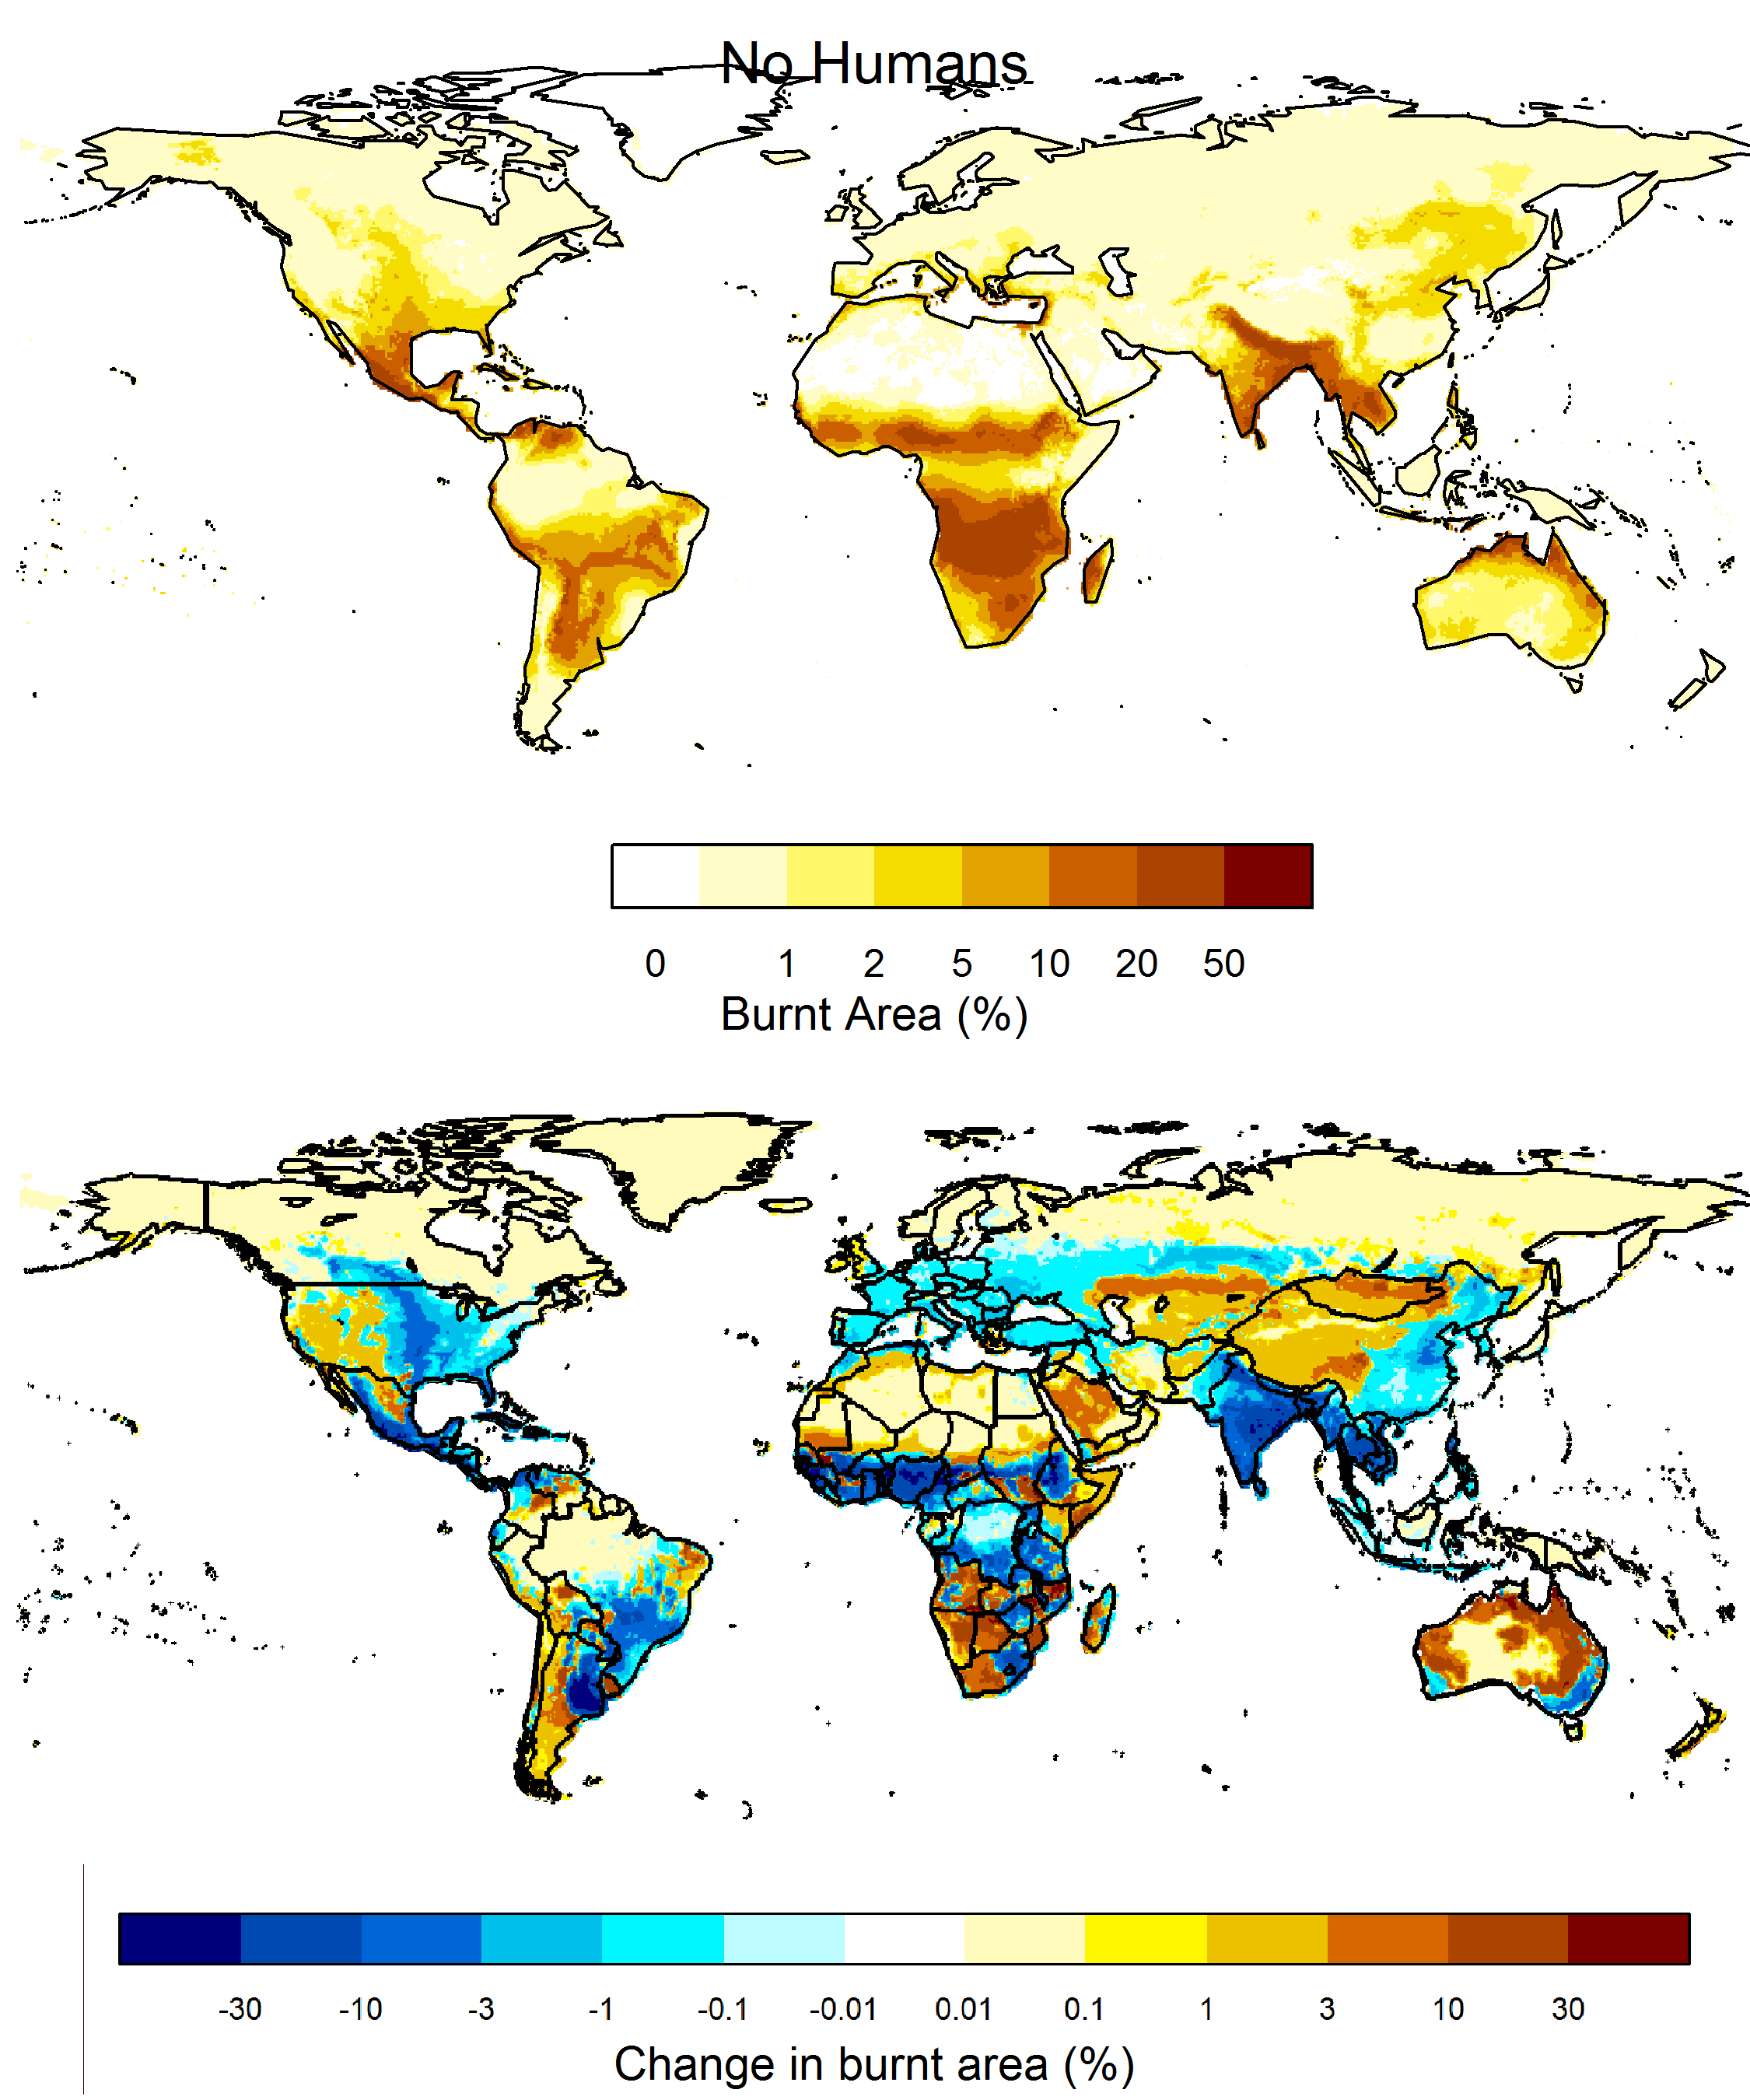
\includegraphics[trim={0 0 0 8cm},clip,width=11.0cm]{images/igntitions/IgntionInfoNoHumans}
    %        };
    %
            %\visible<-1> {\draw[white, fill = white] (5.5,4) -- (12.0,4) -- (12.0,0.0) -- (5.5,0.0) -- (5.5,4);}
    %    \end{tikzpicture}
    %}
\end{frame}

\pgfdeclareimage[width=1.0\paperwidth]{header-image}{header_images/firefighter}

\begin{frame}<2-3>
    \frametitle{Sensitivity to Controls}
    \controlsSide{limitation_map}
\end{frame}
